\chapter{Grundlagen}
In diesem Kapitel sollen die für das weitere Verständnis notwendigen theoretischen Grundlagen erläutert werden. Dazu gehört zunächst der Aufbau des Netzwerks in einem Fahrzeug. Des Weiteren werden relevante Grundlagen der Cyber Security erklärt.

\section{Automotive Networking}
Im Inneren von Autos befinden sich heutzutage eine Vielzahl elektronischer Systeme, von denen jedes mit benachbarten Komponenten kommunizieren kann. Die einzelnen elektronischen Systeme werden als \acp{ECU} bezeichnet. Moderne Autos enthalten in der Regel über 50 verschiedene \acsp{ECU} \cite[vgl.][6]{Miller.2013}. Da diese Kontrolleinheiten zum Teil lebensentscheidende Aufgaben übernehmen, muss die Kommunikation zwischen den Einheiten möglichst in Echtzeit erfolgen. \\

\begin{figure}[H]
\centering
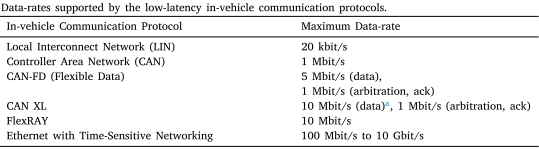
\includegraphics[width=\textwidth]{communication-protocols}
\label{fig:communication-protocols}
\caption{Verschiedene Kommunikationsprotokolle in Automobil-Netzwerken}
\quelle{\cite[2]{MohammadAshjaei.2021}}
\end{figure}

Für die Vernetzung der \acsp{ECU} kommen verschiedene Technologien zum Einsatz (siehe Abbildung \ref{fig:communication-protocols}). Die relevantesten davon werden im Folgenden genauer erläutert. Die wichtigste  davon ist im Automotive-Bereich der sogenannte \acs{CAN}-Standard.

\subsection{Controller Area Network}
Die elektronischen Kontrolleinheiten eines Autos sind typischerweise über einen oder mehrere Busse, die auf dem \ac{CAN}-Standard basieren, miteinander verbunden. Hierbei kommunizieren die \acsp{ECU} über \acs{CAN}-Pakete. Diese werden an alle Komponenten gesendet, welche dann jeweils basierend auf dem Inhalt entscheiden, ob das Paket für sie bestimmt ist oder nicht. Eine Identifikation der Quelle oder Authentisierung gibt es in diesem Standard nicht. \cite[vgl.][7]{Miller.2013} \\
Generell wird meistens zwischen High Speed \acs{CAN} und Low Speed \acs{CAN} unterschieden. High Speed \acs{CAN} wird eingesetzt, wenn bei der Übertragung hohe Geschwindigkeit benötigt wird, beispielsweise bei sicherheitskritischen Anwendungsfällen. Außerdem wird bietet sich die Verwendung von High Speed \acs{CAN} bei der Übertragung von großen Datenmengen an.
In Abbildung \ref{fig:canbus-ford2010} ist das \acs{CAN}-Netzwerk eines 2010 Ford Escape dargestellt. Das abgebildete Netzwerk verfügt über zwei Busse, einen medium speed (MS) und einen high speed (HS) \acs{CAN}-Bus. Beide Busse enden hier im \ac{DLC} (siehe Kapitel \ref{OBD-II}).
In Automotive Netzwerken lassen sich zwei Arten von \acs{CAN}-Paketen finden: normale \acs{CAN}-Pakete und diagnostische \acs{CAN}-Pakete. 

\begin{figure}[H]
\centering
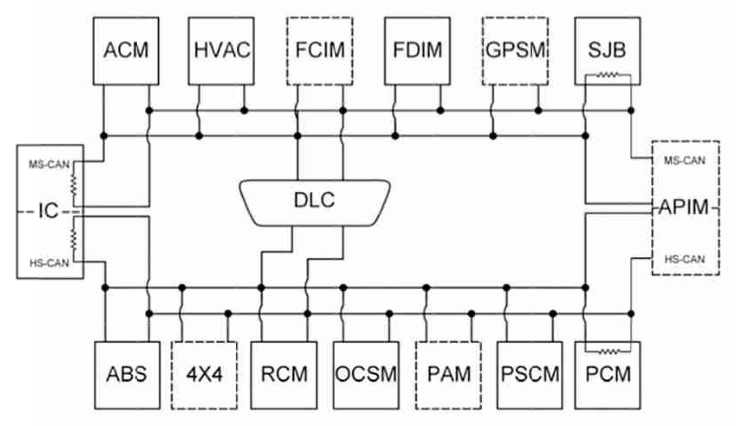
\includegraphics[width=0.7\textwidth]{Miller_canbus-ford2010}
\label{fig:canbus-ford2010}
\caption{Beispiel des \acs{CAN}-Netzwerks eines 2010 Ford Escape}
\quelle{\cite[19]{Miller.2013}}
\end{figure}

\subsubsection{Normale \acs{CAN}-Pakete}
Normale Pakete werden von \acsp{ECU} gesendet und können entweder Informationen oder Befehle enthalten. Typischerweise werden sie alle Millisekunden gesendet. Auf Anwendungsebene enthalten die \acs{CAN}-Pakete einen Identifier, die zu übertragenden Daten und manchmal noch eine Prüfsumme, um sicherzustellen, dass das Paket korrekt übertragen wurde. Der Identifier gibt sowohl an, für welche \acsp{ECU} das Paket bestimmt ist, als auch, welche Priorität das Paket hat. \cite[vgl.][9]{Miller.2013}\\
Das Format einer \acs{CAN}-Botschaft ist in Abbildung \ref{fig:CanBotschaft} dargestellt. Es besteht aus folgenden Bestandteilen:
\subparagraph{Header} CAN ist ein Broadcast-System, bei dem jeder Sender seine Botschaften mit einem eindeutigen Message Identifier markiert.
\subparagraph{Message Identifier} Der Message Identifier kennzeichnet eine Botschaft und dient zur eindeutigen Identifizierung. Er kann entweder 11 Bit (CAN 2.0A) oder 29 Bit (CAN 2.0B) lang sein und enthält zusätzlich 1 bis 3 Steuerbits.
\subparagraph{Control Bits} Die Steuerbits im Control-Feld umfassen den Data Length Code (DLC), der die Anzahl der übertragenen Nutzdatenbytes angibt, sowie eine 15-Bit-Prüfsumme, auch genannt Cyclic Redundancy Check (CRC) zur Fehlererkennung.
\subparagraph{Payload} Die Nutzdaten (Payload) einer Botschaft können zwischen 0 und 8 Datenbytes umfassen.
\subparagraph{Acknowledge und End of Frame} Die CAN-Controller der Empfänger senden eine positive Empfangsbestätigung oder eine Fehlermeldung (Error Frame) innerhalb des Acknowledge und End of Frame Felds.
\subparagraph{Stuffing Bits} Stuffing Bits werden verwendet, um den Bittaktgenerator von Empfängern zu synchronisieren. Sie werden eingefügt, um sicherzustellen, dass nicht mehr als fünf aufeinanderfolgende Bits denselben Wert haben. \cite[61\psqq]{Zimmermann.2014}

\begin{figure}[h]
\centering
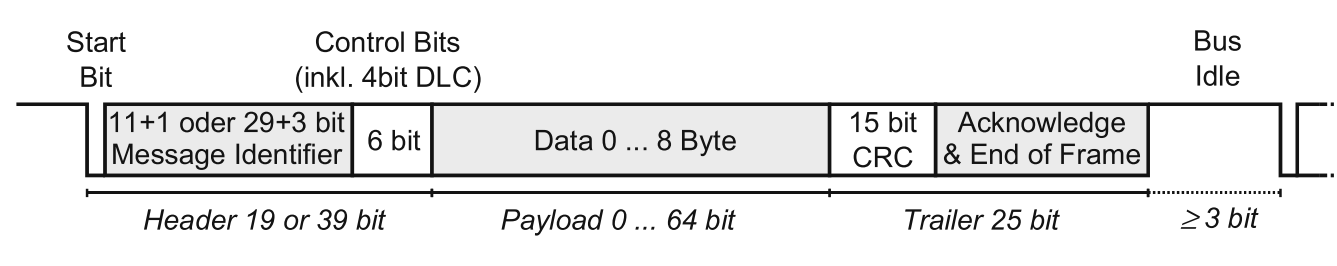
\includegraphics[width=\textwidth]{Zimmermann_CanBotschaft}
\label{fig:CanBotschaft}
\caption{Format einer \acs{CAN}-Botschaft}
\quelle{\cite[61]{Zimmermann.2014}}
\end{figure}


\subsubsection{Diagnostische \acs{CAN}-Pakete}
Diagnostische Pakete tauchen während des normalen Betriebs des Autos im Normalfall nicht auf. Sie werden von Diagnose-Werkzeugen gesendet, die beispielsweise von Mechanikern genutzt werden um mit den \acsp{ECU} im Auto zu kommunizieren. So können Mängel und Fehlfunktionen entdeckt oder andere Informationen gewonnen werden. Das Format von diagnostischen \acs{CAN}-Paketen ähnelt dem von normalen Paketen, erfolgt jedoch meist nach strengeren Konventionen. Standards hierfür sind zum Beispiel ISO-TP, ISO 14229 und ISO 14230. \cite[vgl.][10]{Miller.2013}

\subsection{Local Interconnect Network}
Ein weiteres relevantes Protokoll im Automotive Bereich ist das \ac{LIN} Protokoll. Es wurde 1998 in Zusammenarbeit von Audi, BMW, DaimlerChrysler, Volvo, Volkswagen, VCT und Motorola entwickelt mit dem Ziel, ein möglichst kosteneffizientes Kommunikationsprotokoll zu schaffen \cite[57]{Fijalkowski.2011}.
Das \acs{LIN}-Protokoll basiert auf dem Serial Connections Interface Datenformat und ist in einer Single Master/Multiple Slaves Architektur aufgebaut. Das bedeutet, dass eine elektronische Kontrolleinheit als Masterknoten fungiert und andere elektronische Slave-Einheiten miteinander verbindet.


\subsubsection{Aufbau}
Nachrichtenpakete bestehen im \acs{LIN}-Standard aus einem Header und einem Data Frame. Der Header enthält einen Synchronisation Break, ein Synchronisation Byte und einen Message Identifier. Die ersten beiden Bestandteile sind für die Nachrichtensynchronisierung notwendig. Der Identifier wird benötigt, damit Knoten erkennen können, ob eine Nachricht für sie bestimmt ist. Der Data Frame ist nach dem 8N1-Schema aufgebaut. Das bedeutet, dass jedes Paket ein Startbit, acht Datenbits, kein Paritätsbit und ein Stopbit besitzt. \cite[58]{Fijalkowski.2011} \\
Im \acs{LIN}-Standard sind drei Arten von Kommunikation erlaubt.
\begin{enumerate}
\item Master to Slave, beziehungsweise Master to Multiple Slaves
\item Slave to Master
\item Slave to Slave
\end{enumerate}
Die Slaves können somit auch untereinander ohne Beiteiligung des Masters kommunizieren. \cite[59]{Fijalkowski.2011}

\subsubsection{Anwendung}
\ac{LIN} zeichnet sich wie oben erwähnt vor allem durch seine Kosteneffizienz aus. Allerdings bietet das Protokoll deutlich weniger Bandbreite als \acs{CAN}. Somit wird es vor allem an Stellen im Fahrzeug eingesetzt, wo nicht viel Bandbreite notwendig ist. Beispielsweise wird \acs{LIN} häufig für die Steuerung von Türen, Dach, Sitzen und dem Lenkrad verwendet. \cite[59]{Fijalkowski.2011} \\
Für den Aufbau eines Netzwerks mit den zwei Protokollen gibt es zwei gängige Ansätze:
\begin{enumerate}
\item Mehrere \acsp{ECU} werden über \acs{LIN} mit einer zentralen \acs{ECU} verbunden. Die Verbindung dieser zentralen \acsp{ECU} erfolgt mit dem \acs{CAN}-Standard.
\item Alle \acsp{ECU} werden über \acs{LIN} mit einer zentralen \acs{ECU} verbunden.
\end{enumerate}
Der zweite Ansatz ist skalierbarer, da ohne großen Aufwand neue Knoten hinzugefügt werden können. Der erste Ansatz ermöglicht jedoch eine deutlich höhere Bandbreite bei der Kommunikation zwischen den Einheiten. \cite[58]{Fijalkowski.2011}


\subsection{FlexRay}
Der \ac{CAN} Standard weist neben seinen Stärken auch einige Schwächen auf. Beispielsweise ist die realistisch erreichbare Datenrate beschränkt, zudem lassen sich sehr hohe Datenraten nur mit kurzen Stichverbindungen erreichen. Außerdem verfügt das System nur über einen Kanal und versagt somit bei Ausfall der Busverbindung. Aus diesen Gründen hielten viele Fachleute eine Neuentwicklung für notwendig und sinnvoll \cite[96]{Zimmermann.2014}. Daher wurde FlexRay als Ersatz für \acs{CAN} entwickelt. In der Praxis wird es allerdings größtenteils mehr als Ergänzung als als vollständiger Ersatz eingesetzt \cite[97]{Zimmermann.2014}. Dies könnte an den höheren Kosten aufgrund größerer Komplexität von FlexRay liegen.s FlexRay ermöglicht Aufbauten in Linien- und Sterntopologien. Diese können einkanalig oder zweikanalig sein.\\
Der Aufbau einer FlexRay-Botschaft ist in Abbildung \ref{fig:FlexRayBotschaft} veranschaulicht. Zu Beginn einer FlexRay-Botschaft stehen 5 Steuerbits, in denen Sonderinformationen über die Nachricht angezeigt werden können. Anschließend folgen die Frame ID mit dem Zeitslot der Botschaft, die Nutzdatenlänge, eine Cyclic-Redundancy-Check-Prüfsumme und ein Zykluszähler. 


\begin{figure}[H]
\centering
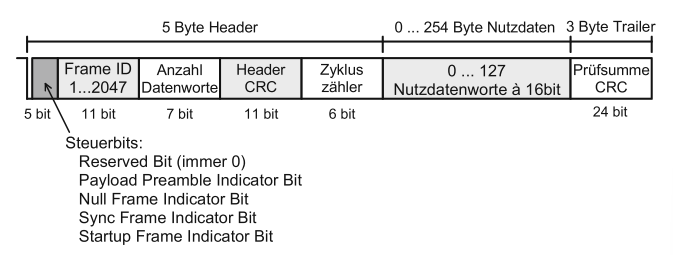
\includegraphics[width=\textwidth]{Zimmermann_FlexrayBotschaft}
\label{fig:FlexRayBotschaft}
\caption{Aufbau einer FlexRay-Botschaft}
\quelle{\cite[101]{Zimmermann.2014}}
\end{figure}


\subsection{Media Oriented System Transport}
Das \ac{MOST} Protokoll wird vor allem in Infotainment-Systemen von Autos eingesetzt. Anstelle von Kabeln werden hier Lichtwellenleiter verwendet. Somit ist das Signal unempfänglich gegenüber elektromagnetischer Einstrahlung. Es wird unterschieden zwischen \acs{MOST}25, \acs{MOST}50 und \acs{MOST}150, welche sich in Paketgröße und Bandbreite unterscheiden. Ein \acs{MOST}-Netzwerk ist meist als Ringtopologie aufgebaut (vergleiche Abbildung \ref{fig:MOST-NetworkMasterSlave}). Auch im \acs{MOST}-Protokoll gibt es Master- und Slave-Knoten. Der Master-Knoten ist häufig ein Gateway zu einem \acs{CAN}-Bus.\\

\begin{figure}[H]
\centering
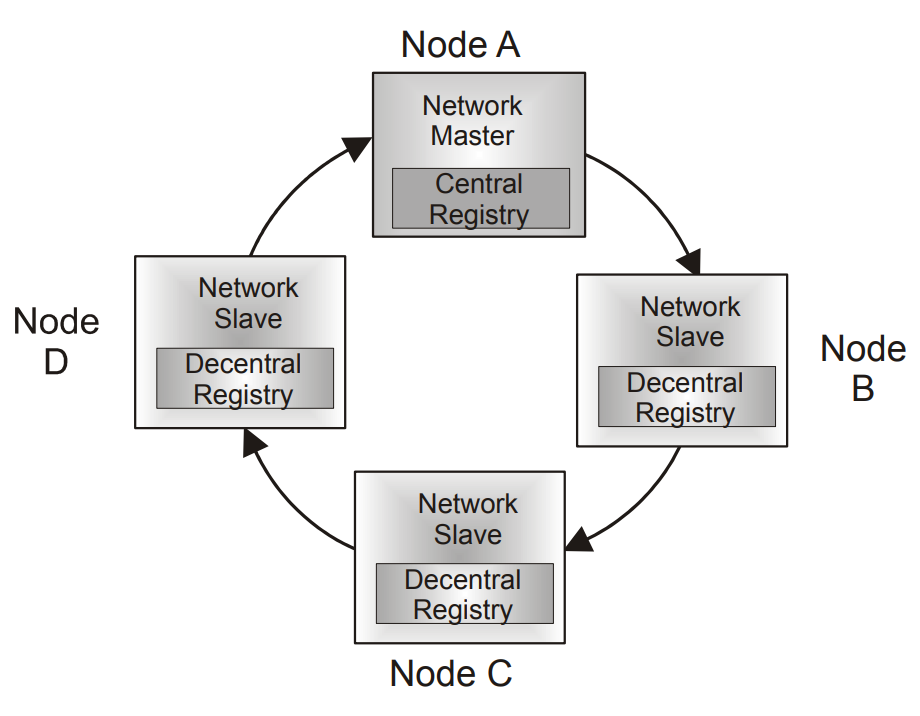
\includegraphics[width=\textwidth]{Grzemba_MOST_NetworkMasterSlave}
\label{fig:MOST-NetworkMasterSlave}
\caption{Ringtopologie eines \acs{MOST}-Bus}
\quelle{\cite[40]{Grzemba.2007}}
\end{figure}

\subsubsection{Paketaufbau}
Der Aufbau eines \acs{MOST}25-Pakets ist in Abbildung \ref{fig:MOST-frame} dargestellt. Es folgt eine kurze Erklärung der Einzelnen Bestandteile.
\subparagraph{Anfangsfeld (Preamble)} Das Anfangsfeld wird vom TimingMaster generiert und dient der Synchronisation der Slaves.
\subparagraph{Abgrenzungsfeld (Boundary Descriptor)}Das Abgrenzungsfeld definiert die in Vier-Byte-Schritten verschiebbare Grenze zwischen Stream- und Paketdaten.
\subparagraph{Datenfeld (stream data, packet data)}Das Datenfeld besteht aus 60 Bytes die nach Bedarf zwischen Streamdaten und Paketdaten aufgeteilt werden können.
\subparagraph{Kontrollbytes (Frame Control)}Die Kontrollbytes am Ende dienen der Kontrolle des Frames.
\subparagraph{Paritätsfeld (Parity Bit)}Das Paritätsfeld ermöglicht das Erkennen von Bit-Fehlern im Frame.
\\

\begin{figure}[H]
\centering
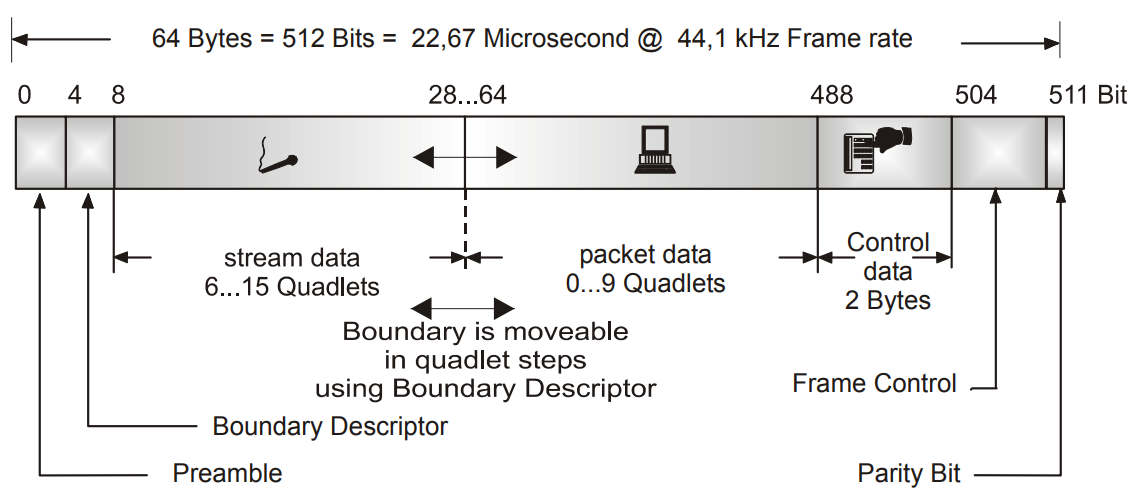
\includegraphics[width=\textwidth]{Grzemba_MOST_frame}
\label{fig:MOST-frame}
\caption{Aufbau eines \acs{MOST}25-Pakets}
\quelle{\cite[88]{Grzemba.2007}}
\end{figure}


\subsection{Automotive Ethernet}
Die Vielzahl inkompatibler und nur in der Automobilindustrie verwendeter Lösungen resultierte in hohen Kosten und kontinuierlichem Weiterentwicklungsaufwand. Zudem steigt der Bandbreitenbedarf. Daher wird das im Bürobereich etablierte Konzept Ethernet/IP relevanter für den Automobilbereich. \cite[138]{Zimmermann.2014}\\
Die in diesem Standard verwendeten Protokolle \ac{IP}, \ac{TCP} und \ac{UDP} werden außerdem bereits von den meisten computerähnlichen Geräten unterstützt. Das ermöglicht eine transparente Kommunikation und vereinfacht die Integration von Consumergeräten erheblich \cite{Zimmermann.2014}. Ethernet war ursprünglich ein Linienbussystem, wird heutzutage aber meistens als Sterntopologie mit Switches an Kopplungspunkten umgesetzt. \\
In Abbildung \ref{fig:EthernetPaket} ist der Aufbau eines Ethernet-Pakets dargestellt. 
Die Präambel und der Start Frame Delimiter spielen eine Rolle bei der Taktsynchronisation bei manchen Physical Layern. Die Ziel- und Quell-MAC-Adresse dienen der Geräteadressierung. Das VLAN-Tag erlaubt die Bildung von Unternetzen. Das Typfeld kennzeichnet den Typ des Inhalts des darauf folgenden Datenfelds. Das Datenfeld enthält den eigentlichen Nachrichteninhalt. Am Ende jedes Pakets befindet sich noch die Frame Check Sequence zur Detektion von Übertragungsfehlern. Beim Eintritt eines Übertragungsfehlers wird die Botschaft automatisch vom Empfänger verworfen. \cite[140]{Zimmermann.2014}\\

\begin{figure}[H]
\centering
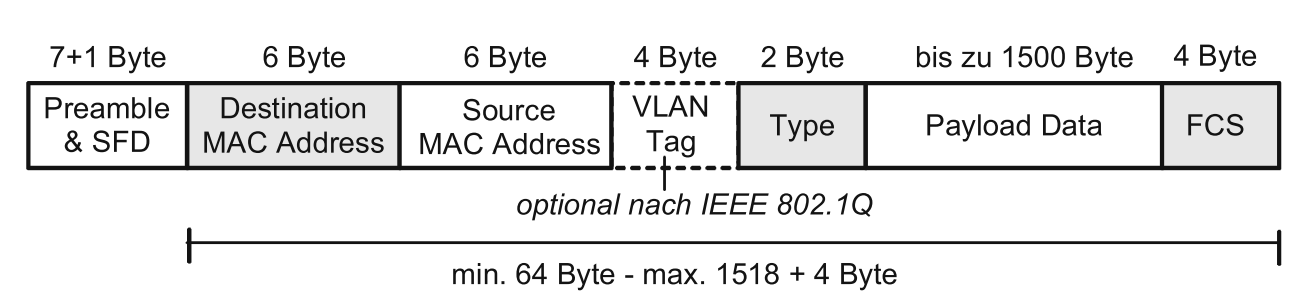
\includegraphics[width=\textwidth]{Zimmermann_EthernetPaket}
\label{fig:EthernetPaket}
\caption{Aufbau eines Ethernet-Pakets}
\quelle{\cite[140]{Zimmermann.2014}}
\end{figure}



\section{Schnittstellen}\label{Schnittstellen}
Moderne Autos verfügen über eine Vielzahl von Schnittstellen, um eine Verbindung mit dem Fahrzeug herzustellen, sei es, um ein Multimediagerät zu verbinden oder zu Diagnosezwecken. Diese Schnittstellen können aber auch eventuell einem potentiellen Angreifer den Zugriff auf das Fahrzeugnetzwerk ermöglichen. Diese möglichen Angriffsvektoren können nach Checkoway et al \cite[1]{Checkoway.2011} in drei Kategorien eingeteilt werden. Diese drei Kategorien sind \glqq indirect physical access\grqq , \glqq short-range physical access\grqq{} und \glqq long-range physical access\grqq . Es folgt eine Beschreibung der Kategorien mit einer Übersicht der typischsten Schnittstellen eines modernen Autos.

\subsection{Indirect Physical Access}
Zu dieser Kategorie zählen sämtliche physische Schnittstellen, die direkt oder indirekt auf die internen Netzwerke des Autos zugreifen. Bei diesen Schnittstellen müsste ein Angreifer, um darauf zuzugreifen, mindestens einmalig physischen Zugang zum Fahrzeug haben oder über einen Vermittler arbeiten. 


\subsubsection{OBD-II Port} \label{OBD-II}
Der \ac{OBD}-II Port ist eine für Fachleute gedachte Schnittstelle auf den \acs{CAN}-Bus zu Diagnosezwecken.	Er befindet sich meist im Fußraum auf der Fahrerseite. Der Port umfasst 16 Pins, obwohl durch den Standard nur die Belegung von neun Pins vorgeschrieben ist. Die zusätzlichen Pins werden je nach Anbieter teilweise für den Zugriff auf zusätzliche Bussysteme verwendet. \cite[2]{Klinedinst.2016} \\
Üblicherweise wird an diesen Port ein Diagnosegerät des Herstellers oder einer Werkstatt angeschlossen. Das Diagnosegerät wird entweder von meist Windows-basierten Personal Computern programmiert oder fungieren als Mittler, um direkt mittels Laptop auf Port zuzugreifen \cite[3]{Checkoway.2011}. In beiden Fällen hat ein Windows-basierter PC direkt oder indirekt Zugriff auf das Netzwerk des Fahrzeugs. Der Hauptzweck dieses Gerätes ist es, Daten aus den \acsp{ECU} des Fahrzeugs zu sammeln. Das erfolgt über das Senden von diagnostischen \acs{CAN}-Paketen. Die betroffenen \acsp{ECU} senden anschließend die angefragten Daten. Diese Daten können dann beispielsweise zur Behandlung von Problemen verwendet werden.\\
Verbrauchermarktanbieter konnten allerdings die Kommunikationsarchitektur durch Reverse-Engineering verstehen und für andere Zwecke nutzen, zum Beispiel Pay-By-Mile-Versicherungen, Fahrzeuggebrauchstracking und kommerzielles Flottenmanagement \cite[3]{Klinedinst.2016}. \\

\subsubsection{Ladeanschluss eines Elektro-Autos}
Elektronische Fahrzeuge tanken nicht an Tankstellen wie ihre kraftstoffbetriebenen Pendants, sondern können an einer Steckdose oder speziellen, teilweise öffentlichen Ladestationen aufgeladen werden. Beim Ladevorgang an Ladestationen werden allerdings nicht nur elektrischer Strom sondern auch Daten ausgetauscht \cite[3]{Checkoway.2011}. Beispiele dafür können die Steuerung des Ladevorgangs, Authentifizierung und Autorisierung und Informationen über Ladezeit, Ladeleistung, Energieverbrauch und Batteriezustand sein. Dieser Datenaustausch ermöglicht einen effizienten und sicheren Ladevorgang, eine Abrechnung des bereitgestellten Stroms und eine Überwachung der Ladeinfrastruktur. Zudem können eine unautorisierte Nutzung der Ladestation oder eine Überlastung des Stromnetzes verhindert werden. 

\subsubsection{Entertainment}
Eine Vielzahl der physischen Schnittstellen eines Autos ist außerdem der Unterhaltung des Benutzers gewidmet. Beispielsweise bieten die meisten Autos mindestens einen USB- und einen Aux-Anschluss, damit Musik von externen Geräten abgespielt werden kann. Außerdem sind viele Autos mit einem CD-Laufwerk ausgestattet. Meist werden mehrere Audioformate unterstützt. Häufig sind die Entertainment-Systeme mit einem \acs{CAN}-Bus verbunden \cite[4]{Checkoway.2011}, um beispielsweise ganzheitliche Firmwareupdates zu ermöglichen. Außerdem kann das Infotainment-System Informationen von anderen Fahrzeugsystemen abrufen, um dem Fahrer relevante Daten anzuzeigen. Dazu gehören Informationen wie Fahrzeuggeschwindigkeit, Motordrehzahl oder Kraftstoffverbrauch, die dann auf dem Display angezeigt werden können.

\subsection{Short-Range Wireless Access}
Diese Kategorie umfasst Schnittstellen, deren Nutzung zwar drahtlos erfolgt, aber dennoch eine geringe physische Distanz zum Fahrzeug erfordert. Ein potenzieller Angreifer müsste sich für die Nutzung dieser Schnittstellen entweder in der Nähe befinden oder einen Transmitter in der Umgebung platzieren.


\subsubsection{Bluetooth}
Um Features wie eine Freisprecheinrichtung oder das Hören eigener Musik vom Smartphone zu realisieren, bieten die Infotainment-Systeme der meisten modernen Autos eine Bluetooth-Schnittstelle. Bluetooth ermöglicht die drahtlose Kommunikation zwischen dem Fahrzeug und externen Geräten wie Smartphones. Durch die Verbindung des Infotainment-Systems mit dem Controller Area Network des Fahrzeugs kann es mit anderen elektronischen Steuergeräten (\acsp{ECU}) kommunizieren. Diese Integration ermöglicht eine nahtlose Interaktion zwischen dem Infotainment-System und anderen Fahrzeugsystemen.
Die Bluetooth-Verbindung eröffnet Möglichkeiten für die Nutzung von verschiedenen Funktionen und Diensten. Eine der häufigsten Anwendungen ist die Freisprecheinrichtung, die es dem Fahrer ermöglicht, Anrufe über das Infotainment-System zu tätigen und entgegenzunehmen, ohne das Telefon in die Hand nehmen zu müssen. Das Infotainment-System wird über Bluetooth mit dem Telefon gekoppelt und kann auf die Telefonkontakte zugreifen, Anrufe initiieren und Anrufinformationen auf dem Display anzeigen.
Darüber hinaus ermöglicht die Bluetooth-Schnittstelle auch die drahtlose Übertragung von Audiodateien vom Smartphone zum Infotainment-System. Fahrer und Insassen können ihre eigenen Musikbibliotheken, Streaming-Dienste oder Podcasts über das Fahrzeuglautsprechersystem abspielen. Das Infotainment-System fungiert als Empfänger für das Audiosignal, das vom Smartphone gesendet wird.

\subsubsection{Remote Keyless Entry}
\ac{RKE} Systeme, auch als Funkfernbedienung oder Keyless-Entry-Systeme bekannt, sind Technologien, die es Fahrzeugbesitzern ermöglichen, ihr Fahrzeug aus der Ferne zu verriegeln und zu entriegeln, ohne einen physischen Schlüssel verwenden zu müssen. Diese Systeme bieten eine bequeme und sichere Möglichkeit, auf das Fahrzeug zuzugreifen.
Ein typisches RKE-System besteht aus zwei Hauptkomponenten: einem Funksender (Fernbedienung) und einem Empfänger, der im Fahrzeug eingebaut ist. Die Fernbedienung ist normalerweise eine kleine tragbare Vorrichtung, die über eine oder mehrere Tasten verfügt. Durch Betätigen der Tasten sendet die Fernbedienung ein verschlüsseltes Funksignal mit einer bestimmten Reichweite an den Empfänger im Fahrzeug.
Der Empfänger im Fahrzeug erkennt das Signal der Fernbedienung und interpretiert es. Wenn das empfangene Signal korrekt und authentifiziert ist, führt das RKE-System die gewünschte Aktion aus. Das kann das Entriegeln oder Verriegeln der Türen, das Aktivieren oder Deaktivieren der Diebstahlalarmanlage oder das Öffnen der Kofferraumklappe sein. In einigen Fahrzeugen können auch weitere Funktionen über die Fernbedienung gesteuert werden, wie das Starten des Motors oder das Ein- und Ausschalten der Fahrzeugbeleuchtung.\\
Des Weiteren sind viele moderne Automobile mit sogenannten Passive Keyless Entry and Start Systemen ausgestattet. Diese basieren auf einem bidirektionalen Challenge-Response-Schema. Das Auto sendet eine Challenge, woraufhin der Autoschlüssel mit einer kryptographischen Antwort (Response) reagiert. Bei einer gültigen Antwort werden die Türen entriegelt, das Alarmsystem deaktiviert und das Starten des Motors ermöglicht. Eine Benutzerinteraktion ist nicht notwendig, der Schlüssel muss sich lediglich in einem Umkreis von in der Regel etwa einem Meter zum Fahrzeug befinden. \cite[930]{Garcia.2016} \\
RKE-Systeme nutzen verschiedene drahtlose Kommunikationstechnologien wie Radiofrequenz (RF) oder Infrarot (IR), um die Signale zwischen der Fernbedienung und dem Fahrzeug zu übertragen \cite[4]{Checkoway.2011}. RF-basierte Systeme sind am weitesten verbreitet, da sie eine größere Reichweite bieten und nicht auf Sichtverbindung angewiesen sind.

\subsubsection{Reifendruck-Kontrollsystem}
Ein weiteres drahtloses Netzwerk in Fahrzeugen stellt das \ac{RDKS} oder auf englisch Tire Pressure Monitoring System (TPMS) dar. Die Integration eines solchen Systems ist in vielen Ländern gesetzlich vorgeschrieben. Neben der Vermeidung von Reifenpannen verspricht die Warnung vor falschem Reifendruck eine Steigerung der Verkehrssicherheit und Kraftstoffeffizienz, da der richtige Reifendruck die Traktion, den Bremsweg und den Rollwiderstand verbessert. Das Reifendrucküberwachungssystem misst kontinuierlich den Luftdruck in allen Reifen von Personenkraftwagen, Lastwagen und Mehrzweckfahrzeugen und warnt den Fahrer, wenn ein Reifen signifikant zu wenig aufgepumpt ist. Es gibt sowohl direkte als auch indirekte Messverfahren. Bei einem direkten Messsystem werden batteriebetriebene Drucksensoren in jedem Reifen verwendet, um den Reifendruck zu messen, und die Daten werden über einen Funkfrequenz (RF)-Sender übertragen, da eine Verkabelung von einem rotierenden Reifen zur elektronischen Steuereinheit des Fahrzeugs schwierig umzusetzen ist. Die empfangende Reifendrucksteuereinheit analysiert die Daten und kann über das \ac{CAN} Ergebnisse oder Befehle an den zentralen Bordcomputer senden, um beispielsweise eine Warnmeldung auf dem Fahrzeugdashboard auszulösen. Indirekte Messsysteme leiten den Druckunterschied zwischen den Reifen aus den Unterschieden in der Rotationsgeschwindigkeit ab, die mithilfe der \ac{ABS}-Sensoren gemessen werden können. Ein Reifen mit niedrigerem Druck muss schneller rotieren, um die gleiche Strecke wie ein Reifen mit höherem Druck zurückzulegen. Die Nachteile dieses Verfahrens sind jedoch eine geringere Genauigkeit, die Kalibrierung durch den Fahrer und die Unfähigkeit, den gleichzeitigen Druckverlust in allen Reifen zu erkennen. Daher werden primär direkte Reifenkontrollsysteme verwendet. \cite[1]{Rouf.2010}

\subsubsection{Wireless LAN}
Viele Hersteller statten ihre modernen Autos heutzutage mit einer \ac{WLAN}-Schnittstelle aus \cite[4]{Checkoway.2011}. Die Technologie wird für verschiedene Anwendungsfälle eingesetzt. Viele moderne Autos sind mit Infotainment-Systemen ausgestattet, die WLAN verwenden, um eine drahtlose Verbindung zum Internet herzustellen. Dadurch können Insassen auf Streaming-Dienste, Musik, Online-Radio, und andere Online-Inhalte zugreifen. \acs{WLAN} ermöglicht auch Over-the-Air-Updates für das Infotainment-System, um Softwareaktualisierungen und neue Funktionen bereitzustellen. Auch für den Rest des Fahrzeugs lassen sich je nach Modell teilweise Softwareupdates über \acs{WLAN} herunterladen. Zum Beispiel die Autos von Tesla bieten dieses Feature. Darüber hinaus ermöglicht \acs{WLAN} den Passagieren im Auto in manchen Fahrzeugen die drahtlose Verbindung ihrer mobilen Geräte wie Smartphones, Tablets und Laptops mit dem Internet.
Schließlich werden \acs{WLAN}-basierte Standards ebenfalls in der Fahrzeug-zu-Fahrzeug-Kommunikation eingesetzt. Diese Art der Kommunikation wird auch Dedicated Short-Range Communications (DSRC) genannt \cite[4]{Checkoway.2011}. Durch den Datenaustausch zwischen Fahrzeugen sollen beispielsweise Kollisionen frühzeitig erkannt und verhindert werden. \\
Um die genannten Features umsetzen zu können, ist größtenteils eine Verbindung der \acs{ECU} mit der \acs{WLAN}-Schnittstelle zum Controller Area Network notwendig. Somit kann in vielen Fahrzeugen auch über \acs{WLAN} theoretisch indirekt auf den \acs{CAN}-Bus zugegriffen werden.



\subsection{Long-Range Wireless Access}
Zu dieser letzten Kategorie zählen alle Zugriffskanäle, die aus großer Entfernung, nämlich mehr als einem Kilometer, zugegriffen werden kann. Immer mehr Autos bieten auch derartige Schnittstellen. Diese lassen sich in zwei Kategorien einteilen: Broadcast Kanäle und Adressierbare Kanäle. \cite[4]{Checkoway.2011}

\subsubsection{Broadcast Kanäle}
Broadcast Kanäle sind Kanäle, die nicht speziell auf ein bestimmtes Fahrzeug ausgerichtet sind, sondern von Empfängern nach Bedarf empfangen werden können. Neben der externen Angriffsfläche können weitreichende Broadcastmedien als Steuerungskanäle attraktiv sein (z. B. zum Auslösen von Angriffen), da sie schwer zuzuordnen sind, mehrere Empfänger gleichzeitig steuern können und Angreifer keine genaue Adressierung ihrer Opfer benötigen.
Das moderne Automobil umfasst eine Vielzahl von Empfängern für weitreichende Signale: \ac{GPS}, Satellitenradio, Digitalradio und das Radio Data System (RDS) und der Traffic Message Channel (TMC), die als digitale Unterträger auf vorhandenen FM-Bändern übertragen werden. Die Reichweite solcher Signale hängt von der Sendeleistung, Modulation, Gelände und Störungen ab. Im Allgemeinen werden diese Kanäle in das Mediasystem eines Autos (Radio, CD-Player, Satellitenempfänger) implementiert, das, wie bereits erwähnt, häufig über interne Automobilnetzwerke Zugriff auf andere wichtige Automotive-ECUs ermöglicht. \cite[4\psq]{Checkoway.2011}

\subsubsection{Adressierbare Kanäle}
Über adressierbare Kanäle lassen sich individuelle Fahrzeuge direkt ansteuern. Die Verbindung erfolgt in der Regel über das Mobilfunknetz.\\
Durch diese Kanäle können viele Funktionen bereitgestellt werden. Dazu gehören die Unterstützung von Sicherheit (Unfallberichterstattung), Diagnose (frühzeitige Warnung bei mechanischen Problemen), Diebstahlschutz (Fernverfolgung und Deaktivierung) und Komfort (Zugriff auf Daten wie Fahrtrichtungen oder Wetterinformationen). \cite[5]{Checkoway.2011} \\
Da diese Kanäle meist eine hohe Bandbreite bieten, über große Distanzen und in beide Richtungen funktionieren und das direkte Ansteuern von individuellen Fahrzeugen ermöglichen, sind diese Schnittstellen für potenzielle Angreifer besonders interessant \cite[5]{Checkoway.2011}.

%evt Automatisiertes/autonomes Fahren

%evt Architektur


\section{Cyber Security}
Als nächstes werden die Grundlagen der Cyber Security und IT Sicherheit erläutert, die im Bereich der Automotive Security relevant sind. Die IT Security befasst sich eher mit der Sicherheit von elektronisch gespeicherten Daten während die Cyber Security diese Sicherheit auf ganze Systeme, Netzwerke und Kommunikation ausweitet.
Die Begriffe Cyber- und IT Security sind jedoch eng miteinander verwandt und werden oft als Synonym verwendet.

\subsection{Security und Safety}
Der deutsche Begriff \glqq Sicherheit\grqq{} ist mehrdeutig, was ihn für eine genaue, technische Definition ungeeignet macht. In der IT-Sicherheit wird zwischen den beiden englischen Begriffen \glqq Safety\grqq{} und \glqq Security\grqq{} unterschieden.
\subparagraph{Safety}
\glqq Der Begriff Safety bezeichnet die funktionale Sicherheit, bzw. die Betriebssicherheit eines Systems. Ein System darf seine Umgebung etwa durch undefiniertes, unzulässiges Verhalten oder Zustände nicht gefährden. Safety schützt somit Mensch und Umwelt vor negativen Einflüssen des Systems, etwa durch Fehlverhalten und Ausfälle.\grqq{} \cite[2]{Wurm.2022}
\subparagraph{Security}
\glqq Der Begriff Security bezeichnet die Informations- und Datensicherheit bzw. die Angriffssicherheit eines Systems. Security umfasst alle Eigenschaften und Maßnahmen, die das System vor absichtlichen und unabsichtlichen Bedrohungen
von außen schützen. Security schützt somit das System vor negativen Einflüssen von Mensch und Umwelt, wie etwa Bedrohungen und Angriffe. Während sich die sog. klassische IT-Security auf die Absicherung der informationstechnischen Systeme eines Unternehmens wie etwa Computer, Server, Netzwerke und Internetanbindungen konzentriert, zielt die Cybersecurity im Kontext des Automotive Bereichs auf die Absicherung deren Produkte ab.\grqq{} \cite[2\psq]{Wurm.2022}\\

Safety bezieht sich somit mehr auf die Sicherheit des Nutzers während sich die Security eines Systems mehr auf die Sicherheit von Daten, Informationen und des Systems an sich fokussiert. Im Automotive-Kontext ist Security in vielen Fällen eine Voraussetzung für die Safety von Fahrzeugen, da durch Security-Maßnahmen verhindert werden soll, dass das Fahrzeug in einen Safety-kritischen Zustand gebracht wird. In anderen Fällen stehen sich Safety- und Security-Ziele aber auch teilweise gegenseitig im Weg. Zum Beispiel kann durch erhöhte Security-Maßnahmen die Latenz der Fahrzeugsysteme ansteigen, was sich wiederum negativ auf die Safety auswirkt. Daher kann es eine Herausforderung sein, beide Disziplinen gemeinsam ausreichend zu behandeln.

%evt Authentisierung, Authentifizierung, Autorisierung
\subsection{Sicherheitsziele}\label{Sicherheitsziele}
Die Sicherheitsziele beschreiben Eigenschaften von Informationen und anderen schützenswerten Ressourcen, die gewünscht sind, um Sicherheit zu gewährleisten. Security-Maßnahmen sollten darauf ausgelegt sein, diese Ziele zu erreichen. Faktoren, die das Erreichen der Sicherheitsziele gefährden, können als Bedrohung identifiziert werden. Die klassischen Sicherheitsziele in der IT Security sind Vertraulichkeit, Integrität und Verfügbarkeit (siehe Abbildung \ref{fig:Sicherheitsziele}). Diese Ziele werden manchmal auch als CIA-Ziele bezeichnet. CIA entspricht hierbei der Abkürzung der englischen Begriffe Confidentiality, Integrity und Availability. Im Automotive Bereich werden allerdings oft zusätzlich die Ziele Authentizität, Zurechenbarkeit und Schutz der Privatsphäre genannt \cite[6]{Wurm.2022}. \\

\begin{figure}[H]
\centering
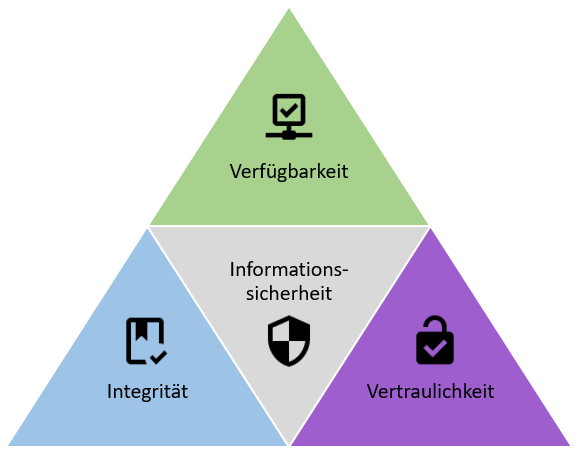
\includegraphics[width=0.5\textwidth]{Sicherheitsziele}
\label{fig:Sicherheitsziele}
\caption{Die drei klassischen Sicherheitsziele der IT Security}
\quelle{\cite{Pukies.2020}}
\end{figure}

\subsubsection{Vertraulichkeit}
\glqq  Vertraulichkeit beschreibt die Eigenschaft, dass ausschließlich berechtigte Personen bzw. Entitäten auf die zu schützenden Informationen zugreifen können.
\grqq{} \cite[7]{Wurm.2022}\\
Dieses Sicherheitsziel kann durch unterschiedliche Maßnahmen erreicht werden, die sich teilweise gegenseitig ergänzen. Dazu gehören zum Beispiel Zugriffskontrollen, Verschlüsselung und Verstecken der Informationen.\\
Es kann verschiedene Gründe geben, warum manche Informationen vertraulich bleiben sollen. So kann durch das Bekanntwerden gewisser Informationen zum Beispiel ein wirtschaftlicher Schaden entstehen. Das kann der Fall sein bei geistigem Eigentum oder auch Firmengeheimnissen. Außerdem schützenswert sind personenbezogene Daten.

\subsubsection{Integrität}
\glqq Integrität beschreibt den Schutz von Informationen vor unbeabsichtigten oder böswilligen Veränderungen.
\grqq{} \cite[7]{Wurm.2022} \\
Das Wort Veränderungen schließt hierbei auch das Entfernen oder Hinzufügen von Daten ein, somit gelten diese Aktionen ebenfalls als Verletzung der Integrität.
Um die Integrität schützenswerter Informationen zu gewährleisten, werden technische Maßnahmen wie kryptographische Checksummen eingesetzt. Dadurch kann zwar ein Verlust der Integrität nicht verhindert werden, jedoch kann er zweifelsfrei und nicht kompromittierbar erkannt werden. Der Schutz der Integrität spielt eine entscheidende Rolle für die korrekte Funktionsweise der gesamten ECU-Software und insbesondere für sicherheitsrelevante Informationen.

\subsubsection{Verfügbarkeit}
\glqq Verfügbarkeit (engl. availability) definiert die Anforderung an das System, seine Dienste und Funktionen innerhalb einer gewissen Zeitspanne (Echtzeitfähigkeit) nach Aufforderung zur Verfügung stellen zu können.
\grqq{} \cite[7]{Wurm.2022} \\
Um einen reibungslosen und sofortigen, teilweise sogar Echtzeit-, Betrieb zu gewährleisten, müssen Hardware-, Software- und Kommunikationsressourcen verfügbar sein. Häufig ist das Ziel eines Angreifers, den Dienst einzuschränken oder vollständig zu verweigern. Eine gängige technische Lösung zur Aufrechterhaltung der Verfügbarkeit ist zum Beispiel die Implementierung redundanter Pfade. Wenn ein Primärsystem ausfällt, kann ein redundantes (Teil-)System die Aufgabe übernehmen und so die Verfügbarkeit sicherstellen.

\subsubsection{Authentizität}
\glqq  Authentizität bedingt, dass die Echtheit einer Information bzw. eines Absenders sichergestellt ist. Die Authentizität einer Information ist gegeben, falls dessen Urheber eindeutig identifizierbar und dessen Urheberschaft kryptographisch sicher überprüfbar ist.
\grqq{} \cite[7]{Wurm.2022} \\
Die Authentizität von Informationen ist eng mit der Integrität von Informationen verwandt. Technisch kann Authentizität durch digitale Signatur oder Zertifikate umgesetzt werden.

\subsubsection{Zurechenbarkeit}
\glqq Zurechenbarkeit bzw. Verbindlichkeit (engl. accountability) ist eine Eigenschaft, die dafür garantiert, dass die entsprechende Person oder Entität die Urheberschaft einer bestimmten Information bzw. eine bestimmte Aktion nicht von sich weisen kann.
\grqq{} \cite[8]{Wurm.2022} \\
Der Begriff Nichtabstreitbarkeit wird oft ähnlich verwendet, spielt jedoch insbesondere in rechtlichen Angelegenheiten wie Haftung und Gewährleistung eine Rolle. Es wurde festgestellt, dass die Abstreitbarkeit eine potenzielle Schwachstelle darstellt. Wenn zum Beispiel der Empfang oder das Senden bestimmter kritischer Nachrichten, wie Warnungen vor Stauenden oder Geschwindigkeitsbegrenzungen, bestritten werden kann, ist eine rechtssichere Zuordnung nicht möglich und eine mögliche Strafverfolgung wird erschwert. Ohne das Schutzziel der Nichtabstreitbarkeit könnte jeder Teilnehmer bestreiten, eine bestimmte Nachricht gesendet oder empfangen zu haben. Die technische Umsetzung kann durch manipulationssichere Log-Speicher erfolgen, die den Empfang bestimmter Nachrichten protokollieren und nachweisen können. Die Nichtabstreitbarkeit der Urheberschaft einer gesendeten Nachricht wird durch das digitale Signaturverfahren in Verbindung mit einer vertrauenswürdigen Public-Key-Infrastruktur gewährleistet. \cite[8]{Wurm.2022}

\subsubsection{Schutz der Privatsphäre}
Moderne Fahrzeuge und Hersteller erheben, verarbeiten und speichern personenbezogene Daten. Beispielsweise wird die Position des Autos im Rahmen der \ac{V2X}-Kommunikation zyklisch veröffentlicht. Hierbei ist es zum einen im Interesse der betroffenen Person, des Fahrers, dass sich diese Daten sich nicht zu den betroffenen Personen zuordnen lassen. Außerdem ist es aber auch durch die Datenschutzgrundverordnung, die im Jahr 2018 in Kraft trat. Technisch lässt sich der Schutz der Privatsphäre zum Beispiel mit einer Tarnidentität umsetzen.


\subsection{Risikomanagement}
Der systematische Umgang mit Gefahren und Risiken ist ein wichtiger Bestandteil des Cybersecurity-Engineering-Prozesses. Im Kontext von Cybersecurity-Angriffen beziehen sich Bedrohungen, Schwachstellen und Risiken auf verschiedene Aspekte. Die schützenswerten Güter eines Systems, auch genannt Assets, können sowohl materieller als auch immaterieller Natur sein, wie zum Beispiel sensible Informationen, Fahrzeugfunktionen, Softwarekomponenten, Hardwarekomponenten, Infrastrukturkomponenten und Kommunikationsverbindungen. Risikobewertungsmodelle definieren die Sicherheitseigenschaften der Assets, wie Vertraulichkeit, Integrität und Verfügbarkeit (vergleiche Kapitel \ref{Sicherheitsziele}), und legen ihren Schutzbedarf fest. \cite[5]{Wurm.2022}\\
Bedrohungen können absichtliche oder unabsichtliche Ereignisse sein, die die Schutzziele der Assets beeinträchtigen können, sei es durch bösartige Aktivitäten von Angreifern oder unvorhersehbare Ereignisse wie Ausfälle oder physische Beschädigungen. \\
Angreifer nutzen vorhandene Schwachstellen aus, um Angriffe durchzuführen und die Assets eines Systems zu bedrohen. Passive Angriffe zielen hierbei auf die Informationsbeschaffung ab, während aktive Angriffe darauf abzielen, die Integrität, Authentizität und Verfügbarkeit des Systems zu beeinträchtigen. \\
Risiken werden im Rahmen einer Risikoanalyse bewertet und sind definiert durch Eintrittswahrscheinlichkeit und potenzielles Schadensausmaß. Schwachstellen erhöhen das Risiko, während Gegenmaßnahmen und Schutzkonzepte das Risiko reduzieren. Gegenmaßnahmen, auch als Sicherheitskontrollen bezeichnet, sollen potenzielle Bedrohungen verhindern und die Wahrscheinlichkeit von Angriffen auf ein akzeptables Niveau reduzieren. Angreifer können aus verschiedenen Personengruppen stammen, von Hobby-Hackern bis hin zu staatlichen Organisationen wie Geheimdiensten. Es ist jedoch auch möglich, dass Angriffe von aktuellen Fahrzeugbesitzern selbst durchgeführt werden, beispielsweise durch das Manipulieren des Kilometerstandes zur Erhöhung des Wiederverkaufswerts eines Fahrzeugs. \cite[5\psq]{Wurm.2022}

\subsubsection{Risikomatrix}
Ein sehr verbreitetes Werkzeug der Risikoanalyse ist die Risikomatrix (siehe Abbildung \ref{fig:Risikomatrix}). Sie dient der Einschätzung und Berechnung von Risiken. Mithilfe einer Risikomatrix kann die Bedeutung und das Ausmaß eines Risikos einfach bestimmt und anschaulich visualisiert werden. In der Regel hat eine Risikomatrix die zwei Dimensionen Eintrittswahrscheinlichkeit und Schadensausmaß. Diese verfügen meist über eine vorher zu definierende, künstliche, ordinale Skalierung. Die Risiken werden dann auf einer Skala von niedrig bis hoch in Bezug auf ihre Wahrscheinlichkeit und Auswirkung eingestuft. Die Wahrscheinlichkeit kann beispielsweise in Kategorien wie selten, gelegentlich, häufig oder sehr häufig unterteilt werden, während die Auswirkung auf Kategorien wie gering, moderat, hoch oder katastrophal abgestuft werden kann. Die einzelnen Felder der Matrix sind meist in verschiedenen Farben eingefärbt. Die genaue Farbverteilung der Felder innerhalb der Matrix ist individuell und kann sich je nach Anwendungsfall unterscheiden. In der Regel sind geringe Risiken grün, mittlere Risiken gelb und große Risiken rot eingefärbt. Wo genau die Grenze gezogen wird ist jedoch dem Ersteller überlassen.
Die Risikobewertung erfolgt durch das Zuweisen eines Wertes oder einer Farbe zu jedem Risiko, abhängig von seiner Position in der Risikomatrix. Für die Berechnung eines Wertes wird meist der Wert der Eintrittswahrscheinlichkeit mit dem Wert des Schadensausmaßes multipliziert. Abhängig von der Klassifikation eines Risikos kann anschließend entschieden werden, wie es zu behandeln ist.
\\

\begin{figure}[H]
\centering
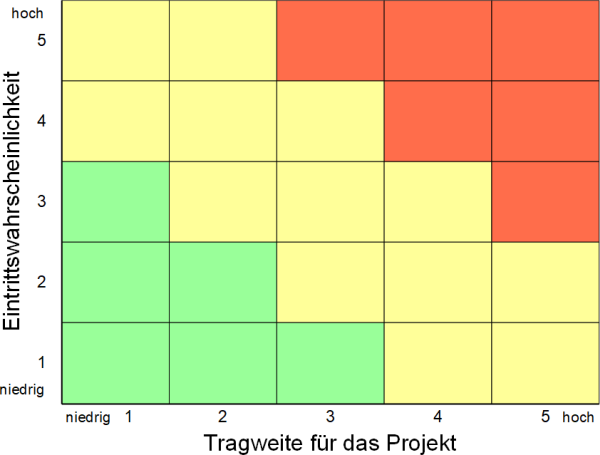
\includegraphics[width=0.7\textwidth]{Risikomatrix}
\label{fig:Risikomatrix}
\caption{Beispiel für eine Risikomatrix}
\quelle{\cite{Peterjohann.2014}}
\end{figure}

%\subsection{ISMS}
%\cite[62]{Wurm.2022} (Kapitel 3)

\subsection{Kryptographie}
\glqq Der Begriff Kryptographie stammt vom griechischen kryptos (verborgen) und graphein (schreiben) ab und bezeichnet die Wissenschaft der Geheimschriften oder der Verschlüsselung von Informationen.
\grqq{} \cite[9]{Wurm.2022}\\
Die Kryptographie beschäftigt sich also hauptsächlich damit, Informationen in anderer Form darzustellen. Dies kann Zwecken der Geheimhaltung, Datenübertragung oder Komprimierung dienen. Außerdem können kryptographische Verfahren wie zum Beispiel RSA auch zur Authentifizierung durch Signaturen eingesetzt werden.\\
Kryptographie im Zusammenhang mit der Sicherheit von Kraftfahrzeugen bezieht sich auf den Einsatz von Ver- und Entschlüsselungstechniken zur Gewährleistung der Vertraulichkeit, Integrität und Authentizität von Daten und Kommunikationssystemen in Fahrzeugen. Durch den Einsatz kryptografischer Techniken werden Informationen vor unbefugtem Zugriff und Manipulationen geschützt, um die Sicherheit und Privatsphäre der Fahrzeuginsassen zu gewährleisten. \\
Hierbei gilt wie in der allgemeinen IT Security das Auguste Kerkhoff Prinzip. Dieses besagt, dass in einem guten Kryptographiesystem lediglich der Schlüssel geheim gehalten werden muss. Das System muss auch dann Sicherheit bieten, wenn seine genaue Funktionsweise bekannt ist. Das Prinzip \glqq Security by Obscurity\grqq , also Sicherheit durch Verschleierung der Funktionsweise des Kryptographiesystems, sollte nicht zum Einsatz kommen. Daher beruhen viele Kryptographieverfahren auf sehr schwer berechenbaren, mathematischen Problemen. Im Fall von RSA wäre das die Faktorisierung sehr großer Zahlen.\\
Im Automobilbereich umfasst die Kryptographie verschiedene Anwendungsfälle, wie die sichere Übertragung von Daten zwischen Fahrzeugkomponenten, die Verschlüsselung von drahtlosen Kommunikationskanälen (z. B. \acs{V2X}-Kommunikation) und die Absicherung von Fahrzeugfunktionen gegen potenzielle Angriffe.
Verschiedene kryptografische Verfahren wie symmetrische und asymmetrische Verschlüsselung, digitale Signaturen und Hash-Funktionen werden eingesetzt, um die Vertraulichkeit von Daten zu gewährleisten, die Integrität von Nachrichten zu garantieren und die Authentizität der Kommunikationsteilnehmer zu überprüfen. Außerdem werden sichere Schlüsselverwaltungssysteme und -protokolle verwendet, um den sicheren Austausch von Verschlüsselungs- und Authentifizierungsschlüsseln zu ermöglichen.
Die Kryptographie spielt im Zusammenhang mit der Sicherheit von Kraftfahrzeugen eine wichtige Rolle, da sie dazu beiträgt, die Risiken von Cyberangriffen auf Fahrzeuge zu verringern und die Sicherheit von Fahrzeugelektronik und Kommunikationssystemen zu erhöhen. Durch den Einsatz kryptografischer Verfahren können vertrauliche Informationen geschützt und die Integrität von Fahrzeugdaten gewährleistet werden, was letztlich zu einer sicheren und zuverlässigen Fahrzeugkommunikation und -funktionalität führt.

%\subsection{Security Lifecycle}
%\cite{Wurm.2022} vlt Kapitel 4


%evt Bedrohungsmodell -> Wurm kapitel 1





\chapter{Angriffsflächen}
Nun da die wichtigsten theoretischen Grundlagen zu Automotive Netzwerken und Cyber Security behandelt wurden, gilt es, die beiden Themenbereiche zusammenzuführen. Hierzu sollen zunächst verschiedene Angriffsflächen von Automobilen untersucht werden. Interessant ist hierbei vor allem, über welche Wege Angreifer sich Zugang zum Fahrzeugnetzwerk verschaffen, wie sie dort ihren Einfluss ausweiten können und wie groß das Risiko für ein Eintreffen des jeweiligen Angriffs ist. 

%\cite[27]{Wurm.2022}
%evt Kapitel 5
%\section{Vorgehen bei der Risikoeinschätzung}


\section{Vernetzte Fahrzeuge aus verschiedenen Perspektiven}
Die zunehmende Vernetzung und Automatisierung im Automobilbereich bedeuten aus Benutzersicht, also aus Sicht der Fahrer und Mitfahrer, vor allem mehr Komfort und ein angenehmeres Fahrerlebnis. Diese Entwicklung ermöglicht viele Features wie Einparkhilfen, Hilfe bei der Parkplatzsuche, Spurhalteassistenten und Frühwarnsysteme vor Staus, Unfällen oder ähnlichem. Solche Features nehmen dem Fahrer Aufgaben ab oder bieten Unterstützung. \\
Aus Hersteller-, Flottenbetreiber oder Verkäufersicht ergeben sich aus der Entwicklung vernetzter und automatisierter Fahrzeuge neue Geschäftsmodelle wie zum Beispiel Car-Sharing, aber auch neue Überwachungs- und Fernkonfigurationsmöglichkeiten der eigenen Fahrzeuge. \\
Aus Angreiferperspektive führt diese Entwicklung hin zu mehr Vernetzung und automatisierung zum Bau von Autos, die von überall aus über das Internet und andere Schnittstellen erreichbar sind, die immer mehr fernsteuerbare Funktionen bieten und die immer mehr ausspähbare Daten über ihre Benutzer erfassen. Das macht moderne Autos zu attraktiven Angriffszielen für mehrere Angreiferarten. Ein Beispiel wären einfache Hobby-Hacker, die gerne ihr Können unter Beweis stellen wollen. Ein weiteres Beispiel sind sogenannte Hacktivisten, die sich unter Umständen gegen den Trend zu mehr Vernetzung und Automatisierung einsetzen wollen. Aber natürlich kann dieses Angriffsziel auch attraktiv auf Hacker mit schlechten Absichten, die ernsthaften Schaden anrichten wollen, wirken.


\section{Charakteristische Vorgehensweise}
Die Art Angriff mit den wahrscheinlich verheerendsten Auswirkungen ist die Kontrollübernahme des Fahrzeugs aus der Ferne. Innerhalb der letzten zehn Jahre haben Whitehat-Hacker mehrfach unter Beweis gestellt, dass eine Fernsteuerung diverser Automobilmodelle über eine Funkverbindung nicht nur theoretisch, sondern auch praktisch möglich ist \cite[35]{Wurm.2022}. Neben dem Jeep Cherokee Angriff von Charlie Miller und Chris Valasek gab es beispielsweise auch erfolgreiche Kompromittierungen von Wagen der Marken BMW und Tesla.\\
In diesen Hackerangriffen zur Fernsteuerung der Zielfahrzeuge sind Gemeinsamkeiten in der Vorgehensweise erkennbar, aus denen sich ein Angriffsmuster ableiten lässt.\\
Der erste Schritt ist der Aufbau einer Verbindung zum Infotainment-System. Dieses ist nicht die einzige angreifbare \acs{ECU}, aber ein sehr praktisches Angriffsziel, da es viele Schnittstellen bietet und oft mit dem \acs{CAN}-Bus verbunden ist.\\
Im zweiten Schritt gilt es, die Kontrolle über das Infotainment-System zu erlangen. Dies gelang den Hackern durch das Ausnutzen verschiedener Schwachstellen.\\
Nachdem die Kontrolle übernommen wurde ist der nächste Schritt der Zugriff auf den \acs{CAN}-Bus über das \acs{CAN}-Gateway. Im Fall des Jeep Cherokee konnte zum Beispiel der Code der Einheit reverse-engineert und umprogrammiert werden.\\
Sobald über das Gateway auf den \acs{CAN}-Bus zugegriffen werden kann, lassen sich von dort aus beliebige \acs{CAN}-Pakete versenden. Das können normale und diagnostische Pakete sein. Ist dieser Punkt erreicht, so hat der Hacker sehr viel Macht über das Fahrzeug und kann verheerenden Schaden anrichten.\\
Schließlich muss dazu allerdings gesagt werden, dass bei sämtlichen dieser Hackerangriffe die Beteiligung zahlreicher Experten und Monate- oder sogar Jahre-lange Vorbereitung für den eigentlichen Angriff notwendig waren. Das Risiko für einen solchen Angriff durch einen gewöhnlichen Hobby-Hacker ist also somit zwar vorhanden, aber nicht sehr wahrscheinlich.


\section{Zugriff}
In diesem Abschnitt erfolgt zunächst eine Untersuchung der teilweise bereits in Kapitel \ref{Schnittstellen} vorgestellten Schnittstellen, über die ein Angreifer sich Zugriff auf das Fahrzeug verschaffen kann. Zudem soll eingeschätzt werden, wie groß das Risiko eines Angriffs über die jeweilige Schnittstelle ist.
%\cite[10]{Miller.2015}


\subsection{Media Player}
Checkoway et al entdeckten Schwachstellen im Media Player eines Autos. So fanden sie heraus, dass der CD-Spieler bei einer speziell formatierten CD nach Anzeigen einer kryptischen Meldung die ganze Einheit mit dem Inhalt der CD neu flasht. Dies bietet die Möglichkeit, eigenen Code in das System einzuschleusen. Des Weiteren stellte sich der Parser für die Audio Dateien als anfällig für einen Buffer-Overflow Angriff heraus. Dem Forscherteam gelang es, eine CD zu erstellen, die die genannten Schwachstellen ausnutzt und beim Abspielen im Media Player \acs{CAN}-Pakete versendet. \cite[7]{Checkoway.2011} \\
Für diese Art von Angriff ist ein Reverse-Engineering der Firmware der Einheit notwendig. Das bedeutet einen großen Aufwand, den jedoch ein ambitionierter Hacker eventuell auf sich nehmen könnte. Erschwerend kommt aber hinzu, dass die entdeckte Schwachstelle nicht bei jedem Media Player funktioniert. Außerdem muss das Opfer des Angriffs zunächst überzeugt werden, die CD abzuspielen. Das Ausmaß des Angriffs ist zwar gefährlich, aber nicht ganz so schlimm wie bei einer Fernsteuerung, da keine Live-Verbindung zum Fahrzeug besteht. Insgesamt ist dieses Risiko daher mittelschwer.

\subsection{OBD-II Port}
Der OBD-II Port bietet direkten Zugriff auf den \acs{CAN}-Bus eines Fahrzeugs. Daher ist das Senden von Paketen über diese Schnittstelle mit weniger Hindernissen verbunden, als wenn zuerst noch eine \acs{ECU} gehackt werden muss. Der Port ist jedoch nur durch direkten physischen Zugriff erreichbar und befindet sich meist im Fußraum des Fahrers. Die Wahrscheinlichkeit, dass sich jemand hier während der Fahrt unbemerkt Zugriff verschafft und die Kontrolle über das Fahrzeug übernimmt, ist sehr gering. Es gibt jedoch noch andere Angriffsarten. Beispielsweise kann der Diagnoselaptop und damit das Diagnosetool einer Werkstatt oder eines Herstellers über das Internet kompromittiert werden. Somit könnte ein Angreifer indirekt aus der Distanz auf den Port zugreifen. Außerdem kann es auch sein, dass sich der Fahrzeugbesitzer selbst unbefugten Zugriff über den Port verschaffen will, zum Beispiel um den Kilometerstand des Fahrzeugs zu ändern und damit den Wert zu steigern. Insgesamt ist die Schwere dieses Risikos bei Betrachtung von Eintrittswahrscheinlichkeit und Schadensausmaß an der Grenze zwischen gering und mittel einzustufen.

\subsection{Bootvorgang}
\cite[82]{Wurm.2022}

\subsection{Passive Anti-Theft System}
Viele moderne Autos haben einen kleinen Chip im Zündschlüssel, der mit den Sensoren des Fahrzeugs kommuniziert. In manchen Fällen ist dieser Sensor direkt mit dem Radio Frequency Hub Module (RFHM) verbunden. Wenn der Zündknopf gedrückt wird, sendet der Fahrzeugcomputer ein RF-Signal, das vom Transponder im Schlüssel empfangen wird. Der Transponder sendet daraufhin ein eindeutiges RF-Signal an den Fahrzeugcomputer zurück und bestätigt damit den Start und die Weiterfahrt. Wenn der Computer nicht den korrekten Identifizierungscode empfängt, bleiben bestimmte Komponenten wie der Anlasser deaktiviert.
Wenn man mögliche Angriffe aus der Ferne betrachtet, ist die Verwundbarkeit dieses Systems minimal. Die einzigen Daten, die von der Software auf dem integrierten Schaltkreis (IC) übertragen und verarbeitet werden, sind der Identifizierungscode und das zugrunde liegende RF-Signal. Es ist schwierig, sich ausnutzbare Schwachstellen in diesem Code vorzustellen. Selbst wenn es welche gäbe, müsste sich ein Angreifer in unmittelbarer Nähe des Sensors aufhalten, da dieser absichtlich so konzipiert ist, dass er nur Signale in der Nähe erkennt.\cite[13]{Miller.2015} \\
Das Risiko eines Angriffs über diese Schnittstelle ist somit zwar theoretisch vorhanden, aber verschwindend gering.


\subsection{Remote Keyless Entry}
\cite{Garcia.2016}

\section{Auswirkung}
\cite[10]{Miller.2015}



\chapter{Schutzmaßnahmen}
\cite[42]{Wurm.2022} und generell Kapitel 2 + 4 + 5
\cite{MillerCharlie.2019}

% Nilsson, D. K. & Larson, U. E. (2009). A defence-in-depth approach to securing the wireless vehicle infrastructure. Journal of Networks, 4(7). https://doi.org/10.4304/jnw.4.7.552-564
%
% Highland, H. J. (1995). AIN’T misbehaving—A taxonomy of anti-intrusion techniques. Computers & Security, 14(7), 606. https://doi.org/10.1016/0167-4048(96)81669-5.



\section{Herausforderungen der Automotive Security}
\cite[36]{Wurm.2022} + 233 (AM-Devices)

\subsection{SecureBoot}
\cite{Wurm.2022}[84]